\section{accessibilita}
Le immagini nel nostro sito risultano essere prevalentemente immagini di contenuto poiche' mostrano effettivamente all'utente come si presenta il nostro centro sportivo all'interno o come si presentano i nostri campi da gioco che andra' a prenotare, abbiamo scelto di assegnare ai tag \textbf{alt} delle immagini frasi del tipo:"il capo da calcetto" poiche' descriverlo risulta impossibile.
\subsection{Accessibilita' per persone affette da daltonismo}
Abbiamo fatto diversi test in internet per testare il nostro sito per le persone che soffrono di daltonismo, qui sotto possiamo vedere qualche immagine filtrata tramite \textbf{http://colorfilter.wickline.org/}
\begin{figure}[H]
	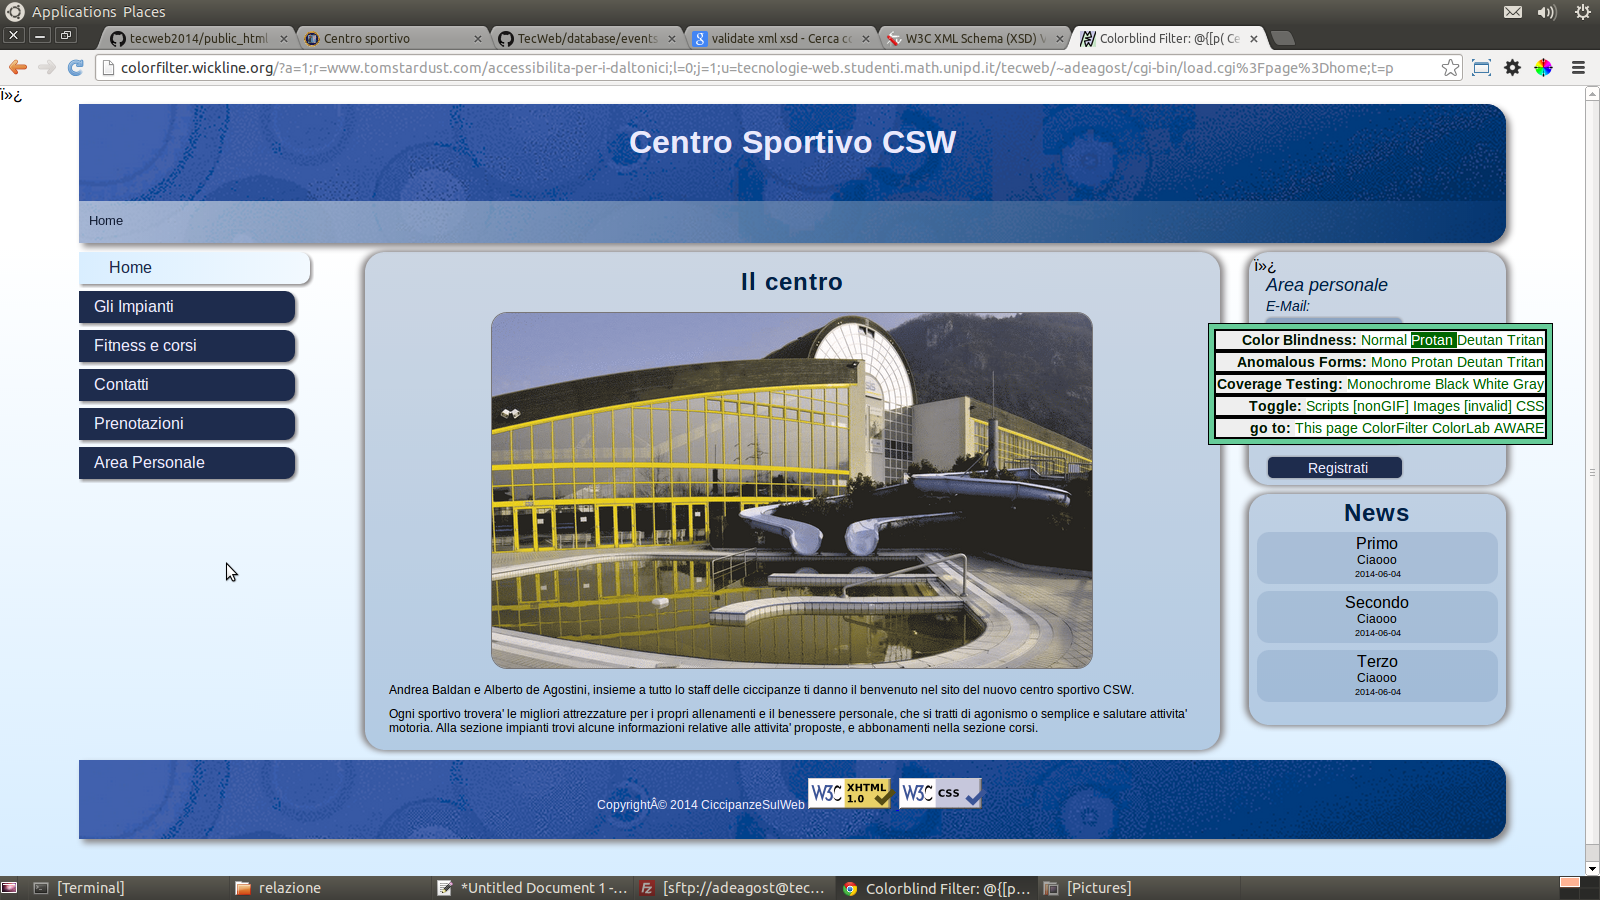
\includegraphics[width=0.8\textwidth]{images/protan.png} 
	\caption{a) protanopia}
\end{figure}
\begin{figure}[H]
	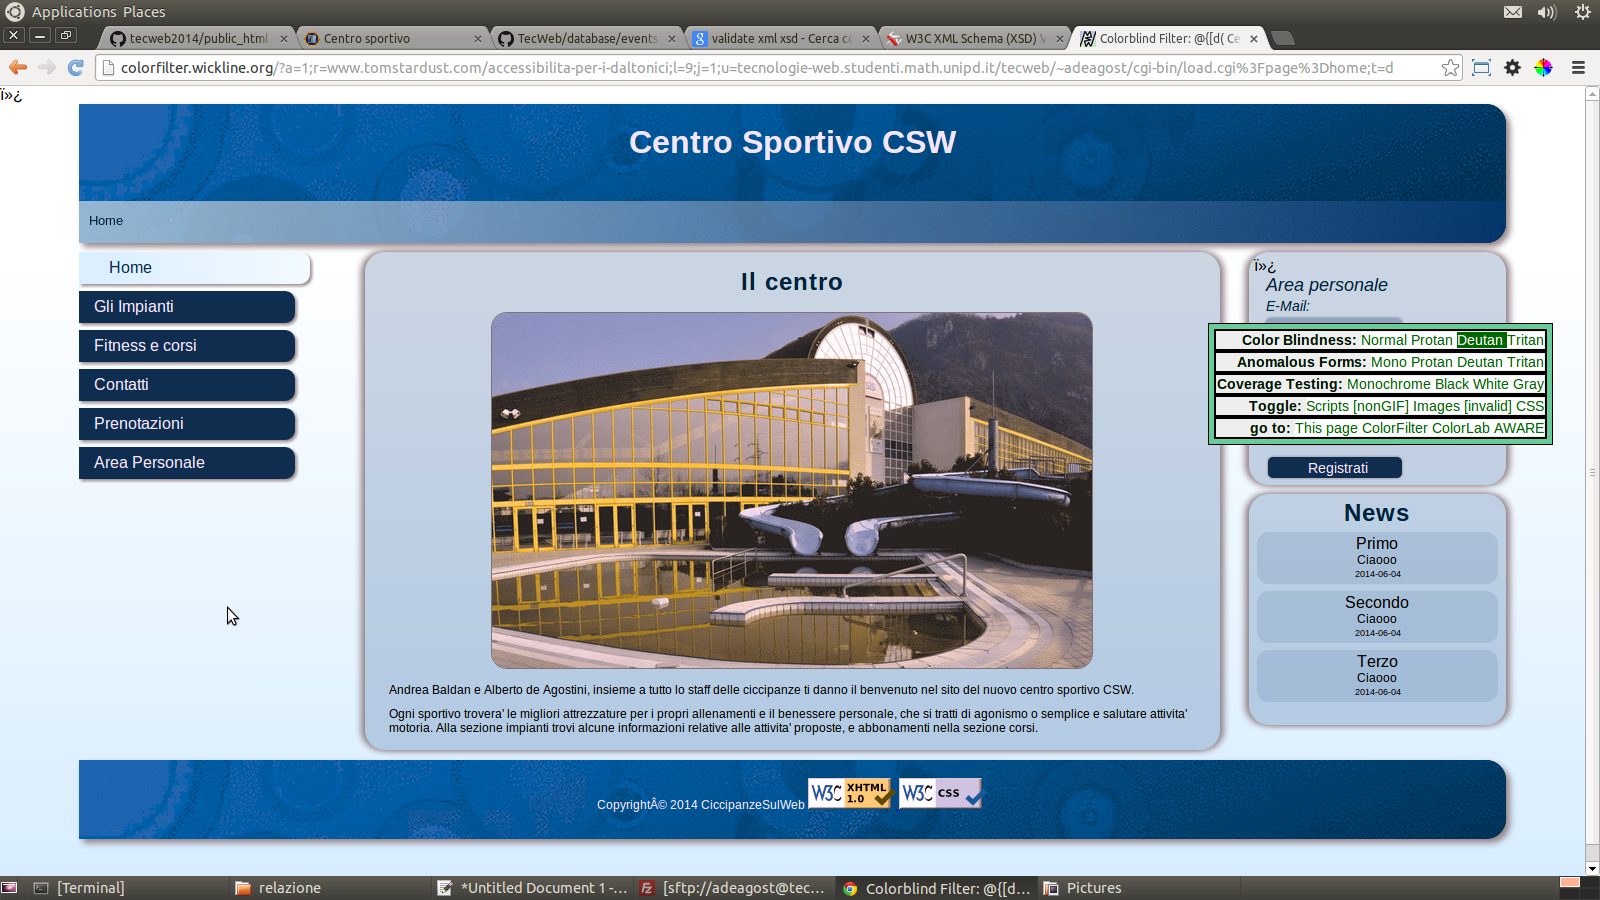
\includegraphics[width=0.8\textwidth]{images/deutran.png} 
	\caption{b) deutranopia} 
\end{figure}
\begin{figure}[H]
	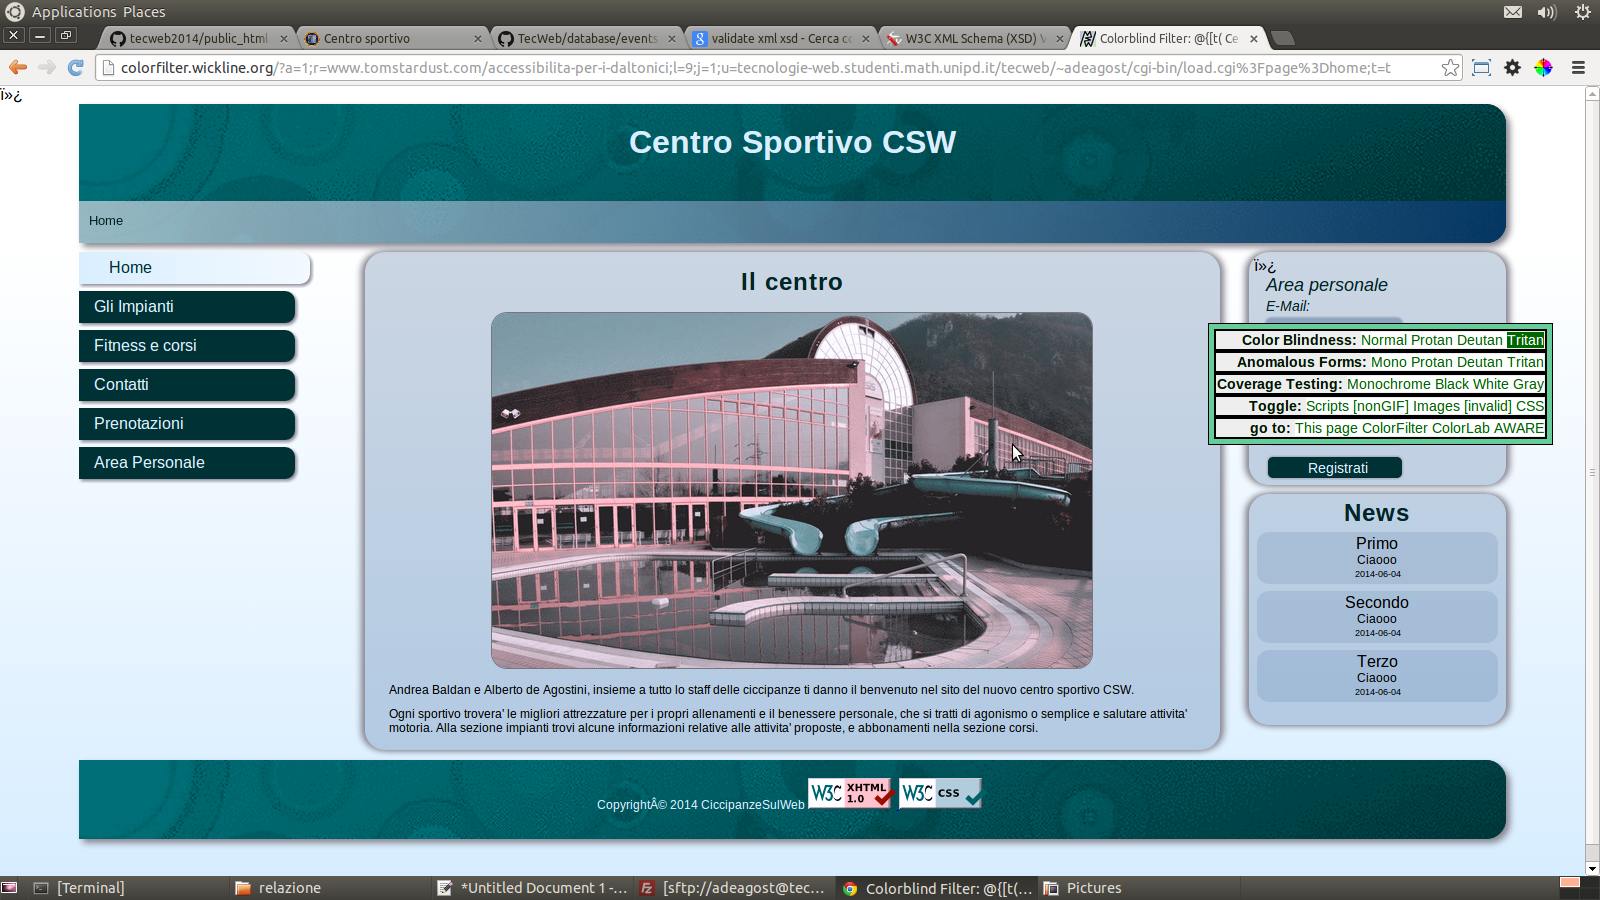
\includegraphics[width=0.8\textwidth]{images/tritan.png} 
	\caption{c) tritanopia}
\end{figure}
abbiamo allegato solo poche immagini visto che i colori utilizzati nel sito sono sempre gli stessi in ogni pagina.\newline
Abbiamo controllato anche il contrasto del sito su \newline \textbf{http://gmazzocato.altervista.org/colorwheel/wheel.php} per scegliere colori con contrasto ratio sempre maggiore di 7 per avere un punteggio di AAA. Su quel sito si puo' vedere anche il contrasto sempre per le persone che soffrono di protanopia, deutranopia e tritanopia.

\subsection{Accessibilita' tramite tastiera}
Un sito per essere accessibile deve essere completamente navigabile anche solo tramite tastiera, la navigazione tramite tastiera nel nostro sito risulta essere lineare e non difficile. Abbiamo inserito prima del \textbf{\#Nav} un link nascosto per saltare direttamente al contenuto per chi non voglia scorrere tutto il menu' di navigazione, lo stesso abbiamo fatto all'inizio del contenuto ove troviamo un altro link nascosto per saltare direttamente al menu' di login cosi' da poter arrivare al menu' login per effettuare l'accesso con soli 2 "salti" per gli utenti che gia' avendo un account vogliono direttamente effettuare un operazione.
Per questi due link nascosti abbiamo utilizzato \texttt{Tabindex} in modo da prioriticizzarli rispetto al resto del sito per favorire una navigazione piu' rapida agli utenti piu' esperti. 
\subsection{Accessibilita' per ciechi}
Abbiamo effettuato test con 4 diversi screen reader:
\begin{itemize}
	\item Jaws
	\item NVDA
	\item Chromevox
	\item Fangs for Firefox
\end{itemize}
La navigazione tramite screen reader risulta essere lineare e non presentare evidenti problemi tuttavia abbiamo notato che ogni screen reader utilizza regole diverse e con qualcuno risulta essere piu' di facile comprensione.
Con NVDA e Jaws abbiamo riscontrato una lettura del sito migliore e una piu' facile navigabilita', con ChromeVox la navigazione ci e' risultata essere piu' difficile tuttavia non e' un vero e proprio screen reader e abbiamo trovato in internet diverse valutazioni negative a riguardo.
Per quanto riguarda Fangs non e' un vero screen reader ma un emulatore di screen reader, ovvero renderizza la pagina come sarebbe letta dallo screen reader dando quindi in output una pagina solamente testuale lineare con le informazioni che sarebbero lette.
Una differenza sostanziale la troviamo quando lo screen reader va a leggere la tablella degli orari dei corsi:\newline
\begin{figure}[H]
	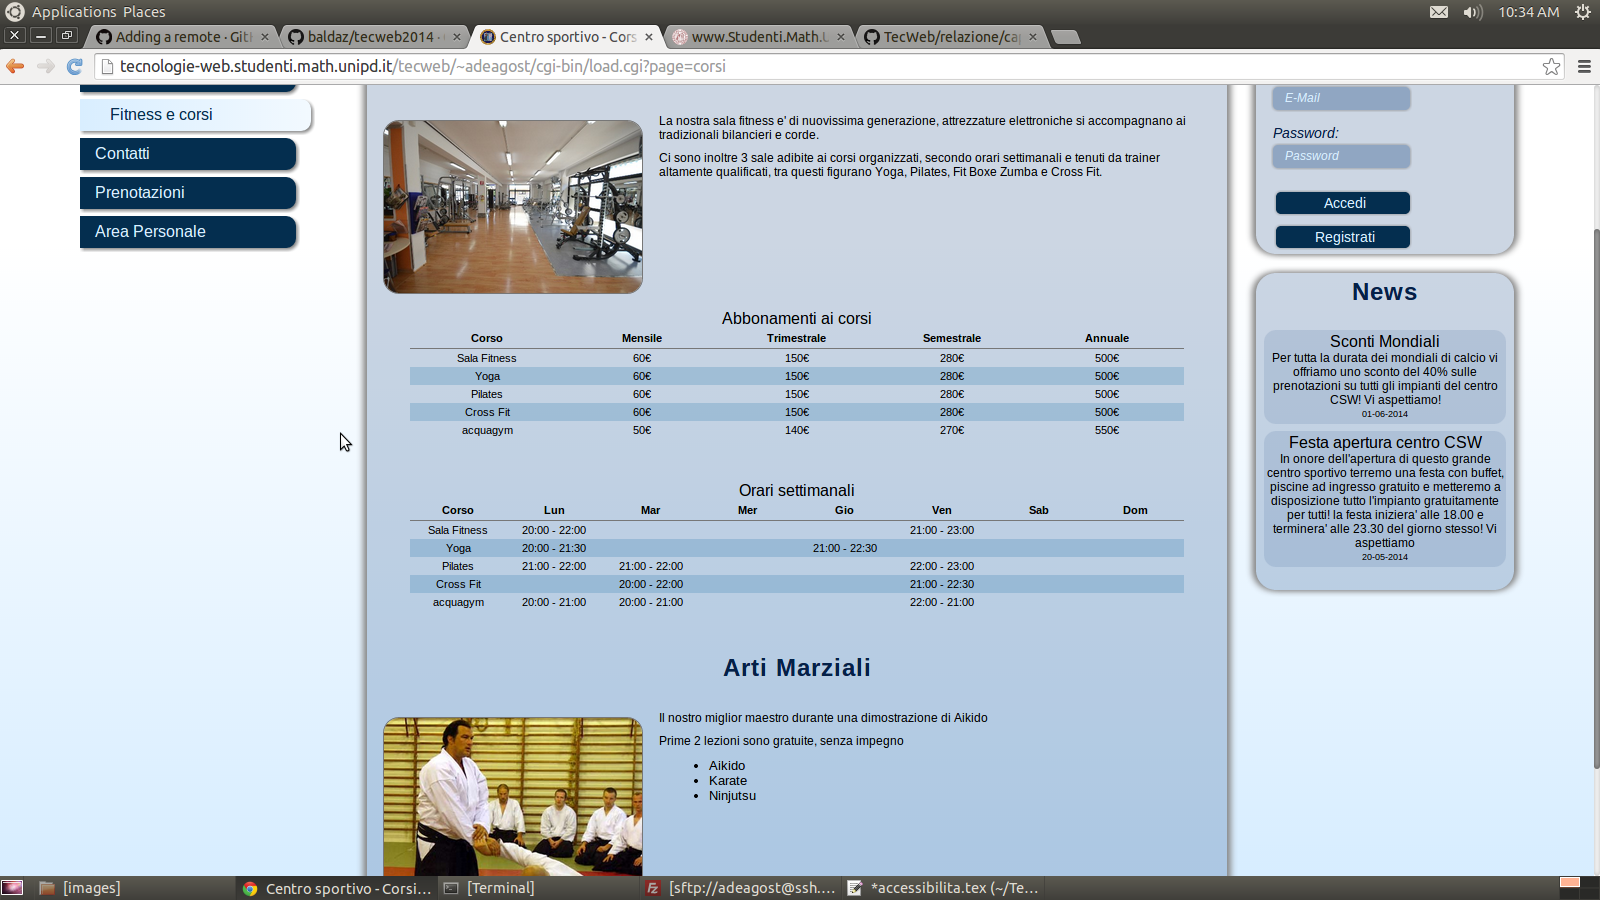
\includegraphics[height=0.4\textwidth]{images/tabella_corsi.png} 
\end{figure}
poiche' con Jaws e NVDA la lettura risulta essere 'giusta' mentre con ChromeVox le caselle vuote vengono saltate compromettendo la comprensione della tabella.
\paragraph{Total Validator}
Abbiamo usato Total Validator per la validazione del nostro sito visto le sue regole stringenti e conformi agli standard WCAG 2.0 AAA. Due errori sono stati riscontrati e non corretti per le motivazioni sottostanti:
\begin{itemize}
	\item Attributo \<time\> non supportato
	\item Attributo \<placeholder\> non supportato
\end{itemize}
Entrambi i tag appena riportati sono stati introdotti in \texttt{HTML5} e percio' non conformi, tuttavia abbiamo deciso di non eliminarli dal sito poiche' entrambi hanno un azione di fallback elegante poiche' quando un browser non supporta \texttt{placeholder} semplicemente o non c'e' testo (placeholder text) nella \texttt{textbox} o il testo e' semplicemente nero.
L'attributo \texttt{time} lo abbiamo lasciato poiche' visualmente non risulta visibile all'utente tuttavia screenreader quali Jaws e NVDA leggono le informazioni interne a \<time\> \</time\> nel modo giusto. 
Esempio "ore \<time\>18:00\</time\>" viene letto 'ore diciotto e zero zero' mentre "ore 18:00" viene letto 'ore diciotto duepunti zero zero' o su alcuni screen reader 'ore milleottocento'.
Per questi motivi abbiamo deciso di lasciare questi tag all'interno nel nostro sito.

\subsection{Accessibilita' parte amministrativa}
La parte amministrativa del nostro sito risulta essere molto semplice e intuitiva.
Abbiamo tralasciato volutamente la parte 'estetica' amministrativa per creare pagine piu' facili da capire.\newline
Tuttavia non abbiamo provato la parte amministrativa con screenreader per mancanza di tempo.
\subsection{Lingua}
Essendo il sito di un centro sportivo locale abbiamo deciso di localizzarlo solamente in lingua italiana.
